\documentclass[aspectratio=169,14pt,usenames,dvipsnames]{beamer}
\usetheme{TalentSprint}
\usepackage[utf8]{inputenc}
\usepackage{graphics}
\usepackage{ragged2e}
\usepackage{amsfonts}
\usepackage{xcolor}
\usepackage{mathtools}
\usepackage{tcolorbox}
\usepackage{setspace}
\usepackage{lmodern}
\definecolor{swe}{rgb}{0.19, 0.73, 0.56}
\definecolor{lgreen}{RGB}{190,200,198}



\begin{document}
\begin{frame}{Focus for this Lecture}

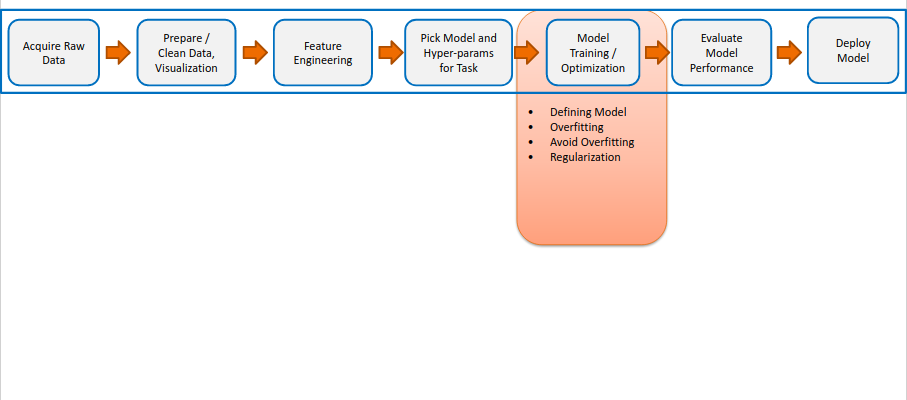
\includegraphics[width=1.0\textwidth, height=0.7\textheight]{Images/AIML_OFG_1.png}
\end{frame}


{\1
\begin{frame} \vspace{35pt}
	\title[Principles and Practice of ML]{Principles and Practice of ML}
	\maketitle
\end{frame}
}


\begin{frame}{What happens when we “train”?}
\begin{itemize}
\item “The problem of training is to find the best W (parameters, coefficients) that minimize the loss/error computed on the training samples”
\end{itemize}

\end{frame}


\begin{frame}{What is the best model?}

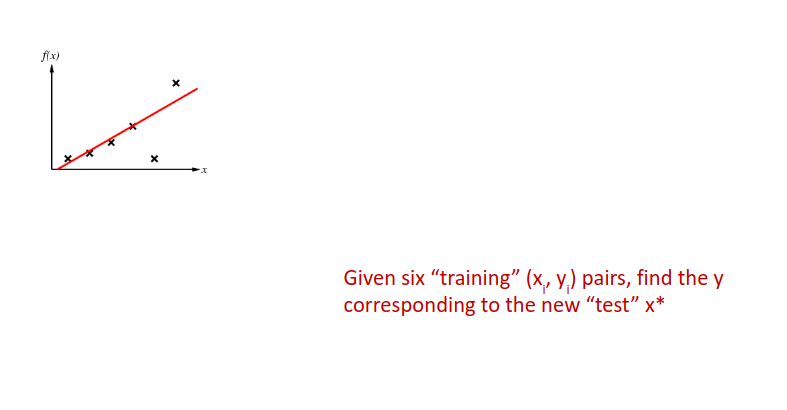
\includegraphics[width=0.9\textwidth, height=0.8\textheight]{Images/AIML_OFG_2.png}

\end{frame}


\begin{frame}{What is the best model?}

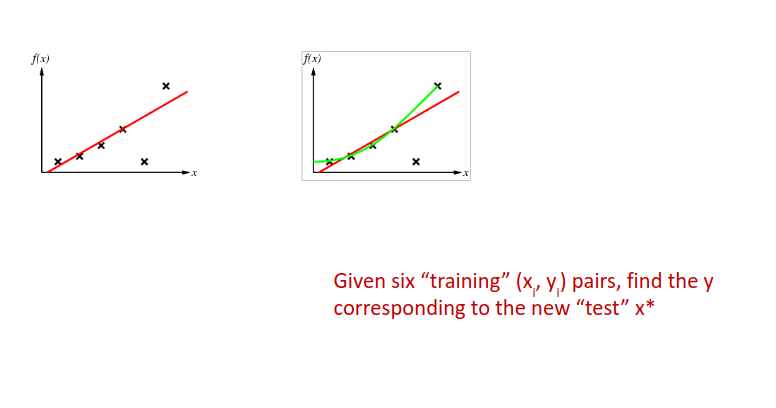
\includegraphics[width=0.9\textwidth, height=0.8\textheight]{Images/AIML_OFG_3.png}

\end{frame}

\begin{frame}{What is the best model?}

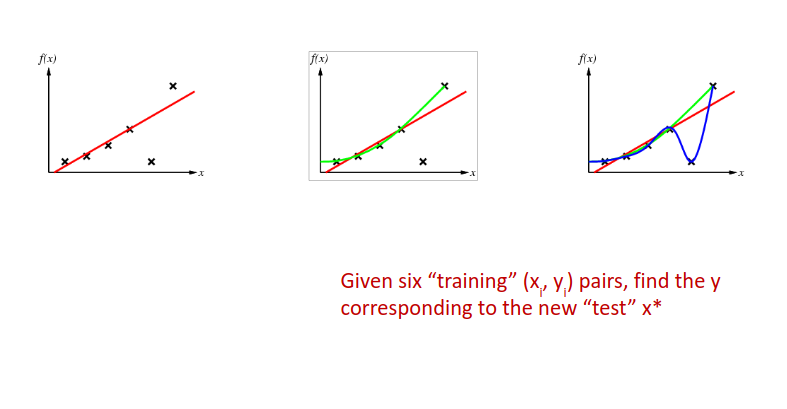
\includegraphics[width=0.9\textwidth, height=0.8\textheight]{Images/AIML_OFG_4.png}

\end{frame}

\begin{frame}{What is the best model?}

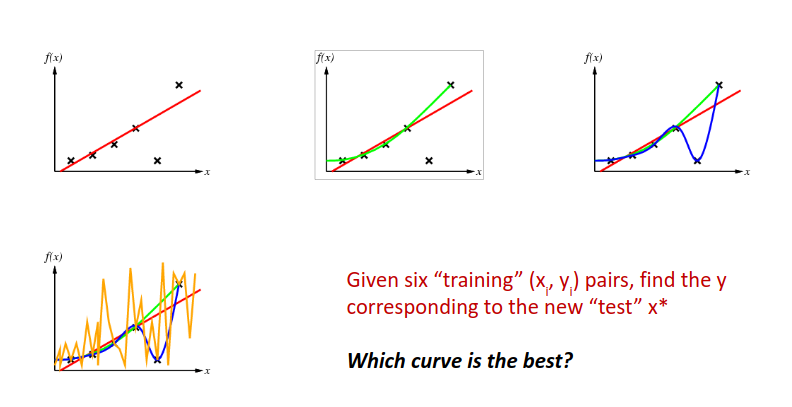
\includegraphics[width=0.9\textwidth, height=0.75\textheight]{Images/AIML_OFG_5.png}

\end{frame}

\begin{frame}{What is the best classifer?}
\centering
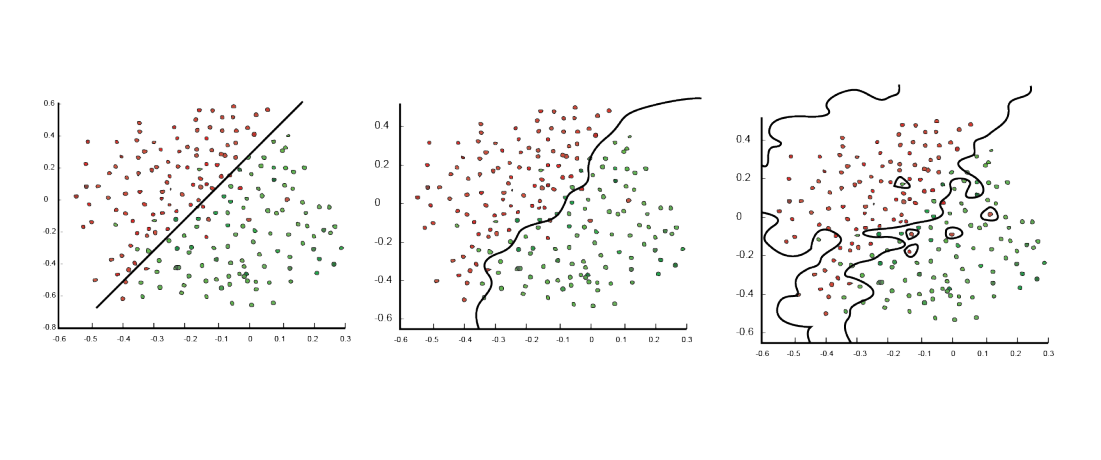
\includegraphics[width=0.8\textwidth, height=0.7\textheight]{Images/AIML_OFG_6.png}

\end{frame}

\begin{frame}{What happens when we simply learn?}
\begin{itemize}
\item We often minimize an error over the training examples.
\item The discrepancy between the actual and predicted. Let xi is the input, zi is the true output and yi is the predicted output. f() is the model, say a Neural Network.

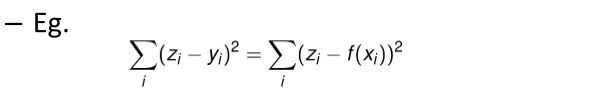
\includegraphics[width=0.5\textwidth, height=0.15\textheight]{Images/AIML_OFG_7.png}

\end{itemize}

\end{frame}


\begin{frame}{What happens when \\ we simply learn? (Cont..)}
\begin{itemize}
\item \alert{If we want only to minimize this, we can even get zero error. The perfect error. }
\item \alert{But we do not want that. \textbf{Then what do we want?}}

\end{itemize}

\end{frame}


\begin{frame}{We know about f() that fits \\ samples perfectly}
\centering
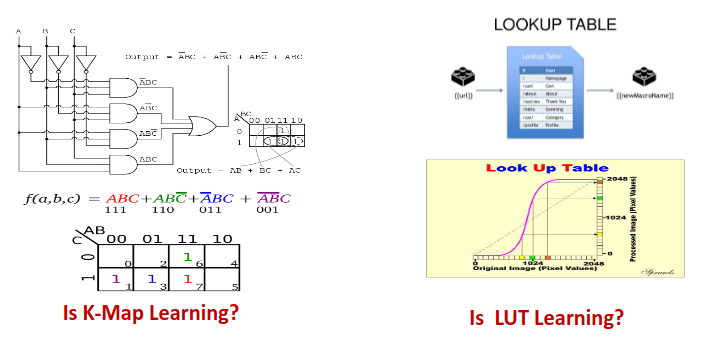
\includegraphics[width=0.8\textwidth, height=0.7\textheight]{Images/AIML_OFG_8.png}

\end{frame}

\begin{frame}{Learning}
\centering
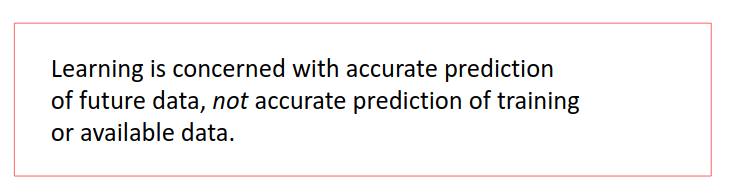
\includegraphics[width=0.9\textwidth, height=0.4\textheight]{Images/AIML_OFG_9.png}

\end{frame}


\begin{frame}{Memorization and generalization}
\begin{itemize}
\item \alert{\textbf{Memorization:}}
\begin{itemize}
\item We are concerned with performance on our limited data. 
\end{itemize}
\end{itemize}

\begin{itemize}
\item \alert{\textbf{Generalization}}
\begin{itemize}
\item Refers to the capability of applying learned knowledge to previously unseen data
\item Without generalization there is no learning, just memorizing!
\end{itemize}
\end{itemize}

\end{frame}

{\1
\begin{frame}
	\title{Questions?}
	\maketitle
\end{frame}}


\begin{frame}{Generalization}
\begin{itemize}

\item We only have “\alert{\textbf{training data}}”. Then how do we minimize error on unseen/future data?
 
\end{itemize}
\end{frame}

\begin{frame}{Occam’s Razor}
\begin{itemize}

\item \alert{\textbf{Select the simplest hypothesis (solution) that suits/fits the data.}} 
 
\begin{itemize}
\item Eg. Minimize Sum of “fit error” and “degree of the polynomial”

\end{itemize}
\end{itemize}
\end{frame}

\begin{frame}{Model Complexity: Examples}
\begin{itemize}

\item This is the complexity of our solution
\item \alert{\textbf{Neural Networks:}} Examples 
 
\begin{itemize}
\item Number of Neurons 
\item Number of Weights 
\item Number of Learnable parameters

\end{itemize}
\end{itemize}

\begin{itemize}
\item \alert{\textbf{Decision Tree:}} Example
 
\begin{itemize}
\item Depth of the tree
\end{itemize}
\end{itemize}

\end{frame}


\begin{frame}{What’s in that we learn from}
\begin{itemize}

\item The data usually has two parts
\begin{itemize}
\item \alert{\textbf{Signal:}} information that is relevant to pattern detection or prediction
\item \alert{\textbf{Noise:}} information that is irrelevant to the future
\end{itemize}
\item Finding which is which is the challenge
\end{itemize}

\centering
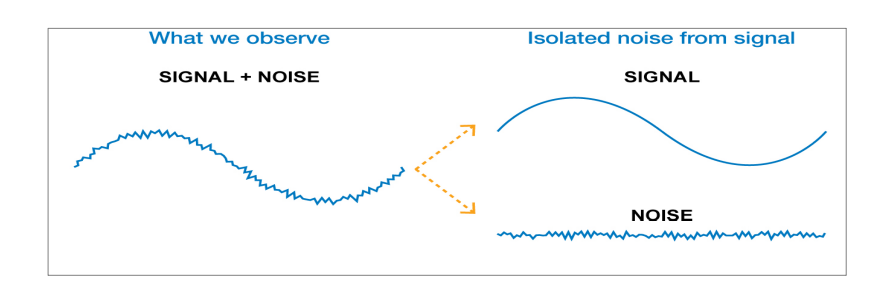
\includegraphics[width=0.65\textwidth, height=0.35\textheight]{Images/AIML_OFG_10.png}

\end{frame}

\begin{frame}{Model the Signal; Not Noise}
\centering
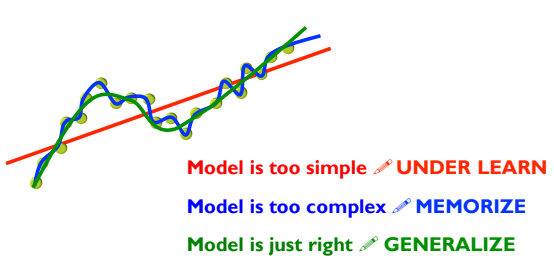
\includegraphics[width=0.6\textwidth, height=0.5\textheight]{Images/AIML_OFG_11.png}
\end{frame}

\begin{frame}{Generalize, Don’t Memorize!}
\centering
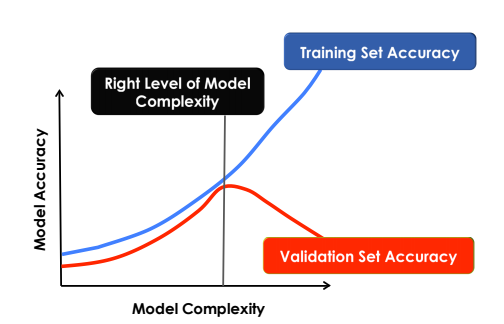
\includegraphics[width=0.55\textwidth, height=0.55\textheight]{Images/AIML_OFG_12.png}
\end{frame}


\begin{frame}{We can plot learning curves \\ to spot overfitting}
\centering
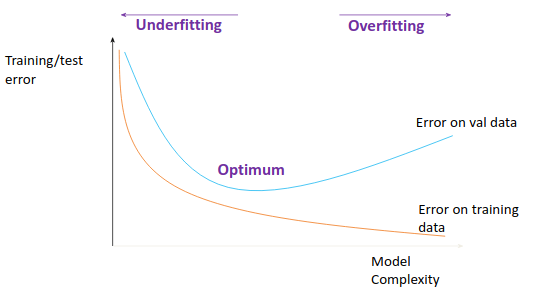
\includegraphics[width=0.55\textwidth, height=0.6\textheight]{Images/AIML_OFG_13.png}
\end{frame}

{\1
\begin{frame}
	\title{Questions?}
	\maketitle
\end{frame}}


\begin{frame}

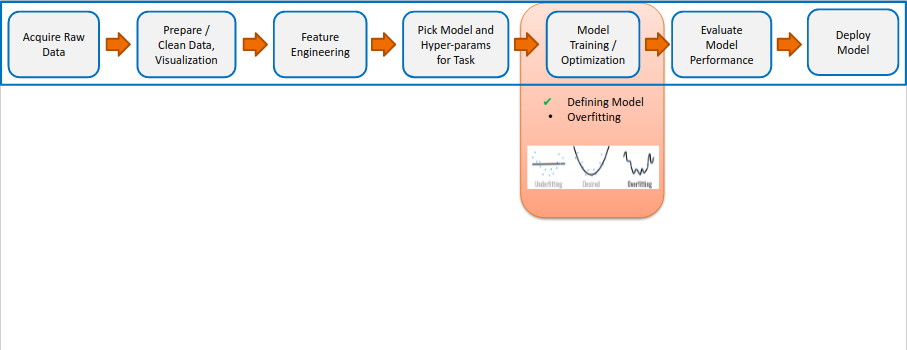
\includegraphics[width=1.0\textwidth, height=0.8\textheight]{Images/AIML_OFG_14.png}
\end{frame}


{\1
\begin{frame} \vspace{35pt}
	\title[Overfitting]{Overfitting}
	\maketitle
\end{frame}
}

\begin{frame}{Overfitting}
\begin{itemize}
\item “Overfitting is a modeling error which occurs when a function is too closely fit to a limited set of data points. Overfitting the model generally takes the form of making an overly complex model to explain idiosyncrasies in the data under study. In reality, the data often studied has some degree of error or random noise within it. Thus attempting to make the model conform too closely to slightly inaccurate data can infect the model with substantial errors and reduce its predictive power.”
\end{itemize}
\end{frame}


\begin{frame}{Simple models cause underfitting}
\begin{columns}
\column{0.7\textwidth}
\begin{itemize}
\item In underfitting, the training error and test error are high
\item What does too simple mean?
\begin{itemize}
\item Too few features
\item Use of features is not ‘complex’
\end{itemize}
\end{itemize}

\begin{itemize}
\item Examples
\begin{itemize}
\item Can you predict well if an email is spam 
\item using only the word ‘free’?
\item Can you predict well housing prices using only the year it was built?
\end{itemize}
\end{itemize}

\column {0.4\textwidth}
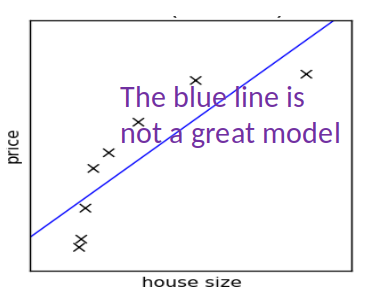
\includegraphics[width=5.5cm, height=5cm]{Images/AIML_OFG_15.png}
\end{columns}
\end{frame}


\begin{frame}{Overfitting is when the model \\ learns the noise and signal}
\begin{columns}
\column{0.7\textwidth}
\begin{itemize}
\item If the model overfits
\begin{itemize}
\item It cannot \alert{generalize} well to new data
\item It \alert{memorizes} the training data
\item It has a \alert{low training error}, and \alert{high test error.}
\end{itemize}
\end{itemize}


\column {0.4\textwidth}
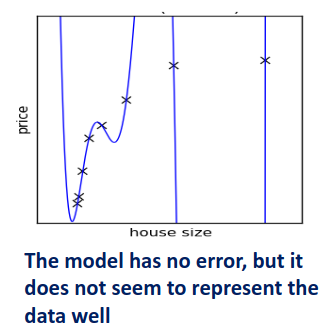
\includegraphics[width=5cm, height=5cm]{Images/AIML_OFG_16.png}
\end{columns}
\end{frame}


\begin{frame}{Overfitting is caused by:}
\begin{itemize}
\item Too much model complexity
\begin{itemize}
\item Typically too many features
\item Too many parameters to learn
\end{itemize}
\item Too little data or not enough data diversity
\end{itemize}
\end{frame}


\begin{frame}{Revisit our favorite question:}
\centering
“What is the ‘best’ parameter for my training data? How do I find the best?”

\end{frame}


{\1
\begin{frame}
	\title{Questions?}
	\maketitle
\end{frame}}


\begin{frame}

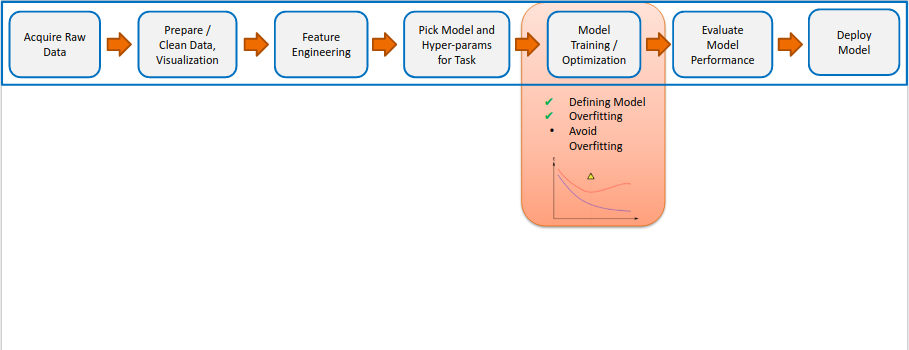
\includegraphics[width=1.0\textwidth, height=0.8\textheight]{Images/AIML_OFG_17.png}
\end{frame}


{\1
\begin{frame} \vspace{35pt}
	\title[Avoiding Overfitting]{Avoiding Overfitting}
	\maketitle
\end{frame}
}

\begin{frame}{Addressing Overfitting}
\begin{itemize}
\item Use More Data $\rightarrow$ Can learn more parameters
\item Reduce the number of features or dimensions
\begin{itemize}
\item Select which features to keep
\item Reduce dimension
\item Select which model to use
\end{itemize}
\end{itemize}
\end{frame}


\begin{frame}{How to prevent/reduce overfitting?}
\begin{itemize}
\item \alert{Train with more data}
\item \alert{Reduce/Remove features}
\item \textbf{Early Stopping}
\item \textbf{Regularization}
\item Ensembling (later)
\end{itemize}
\end{frame}


\begin{frame}{Early Stopping}
\centering
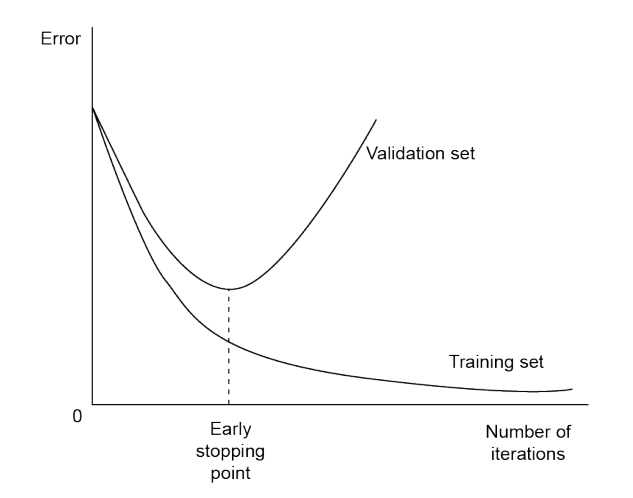
\includegraphics[width=0.5\textwidth, height=0.6\textheight]{Images/AIML_OFG_18.png}
\end{frame}


\begin{frame}

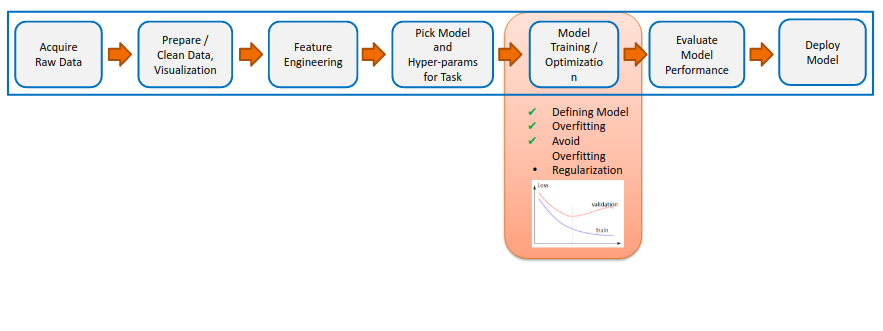
\includegraphics[width=1.015\textwidth, height=0.7\textheight]{Images/AIML_OFG_19.png}
\end{frame}

{\1
\begin{frame} \vspace{35pt}
	\title[Regularization]{Regularization}
	\maketitle
\end{frame}
}

\begin{frame}{Regularization}
\centering
Regularization is a process of introducing additional information in order to solve an ill-posed problem or to prevent overfitting.
\end{frame}

\begin{frame}{What to Minimize? (regularization)}
\begin{itemize}
\item We were minimizing:
\end{itemize}
\centering
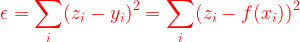
\includegraphics{Images/AIML_OFG_20.png}
\begin{itemize}
\item We can minimize
\end{itemize}
Fit error + some measure of complexity of the model \\
\centering
$\alert{\epsilon}$ + Sum of squares of Weights \\
\centering
$\alert{\epsilon}$ + Number of Non-zero Weights
\end{frame}


{\1
\begin{frame} \vspace{35pt}
	\title[Effect of Regularization]{Effect of Regularization}
	\subtitle{Casestudy}
	\maketitle
\end{frame}
}


\begin{frame}[t]{\hspace{3ex} Fit a curve to the data}
\begin{columns}
\begin{tikzpicture}[remember picture,overlay]
\node[anchor=north west,xshift=-10pt,yshift=11pt] at (current page.north west) {
\includegraphics[height=2cm]{Images/AIML_OFG_23.png}};
\end{tikzpicture}
\column{0.6\textwidth}

\begin{itemize}
\item Learn W to fit the following polynomial to data using regression
\end{itemize} 
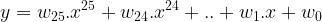
\includegraphics{Images/AIML_OFG_25.png}

\column {0.4\textwidth}
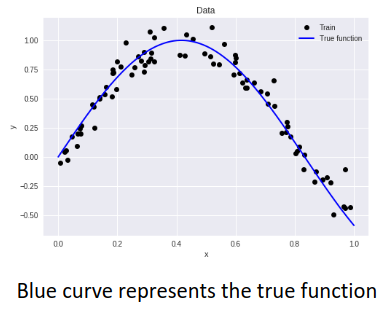
\includegraphics[width=5.5cm, height=5cm]{Images/AIML_OFG_21.png}
\end{columns}

\end{frame}


\begin{frame}[t]{\hspace{3ex} Curve fitting with different \\   regularizations}

\begin{tikzpicture}[remember picture,overlay]
\node[anchor=north west,xshift=-10pt,yshift=11pt] at (current page.north west) {
\includegraphics[height=2cm]{Images/AIML_OFG_23.png}};
\end{tikzpicture}

\centering
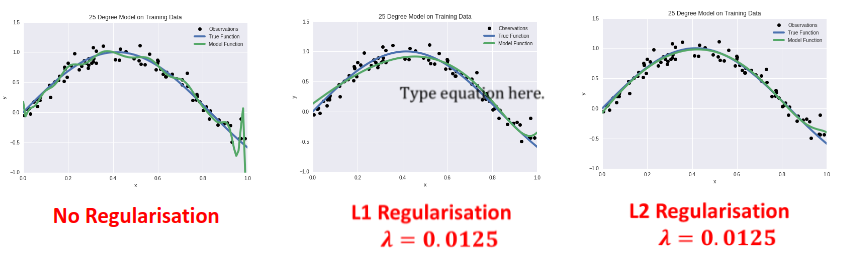
\includegraphics[width=12.5cm, height=5cm]{Images/AIML_OFG_22.png}

\end{frame}


\begin{frame}{Summary}
\begin{itemize}
\item Find model that is simple and fitting the data.
\item Problem of overfitting.
\begin{itemize}
\item How to detect? What to observe during learning?
\item How to avoid.
\end{itemize}
\end{itemize}
\begin{itemize}
\item Regularize the solution by adding extra term that also minimize the “complexity”.
\item Right way to design solution with

\begin{itemize}
\item Train, Val and Test splits.
\end{itemize}
\end{itemize}
\end{frame}


\begin{frame}{Summary}

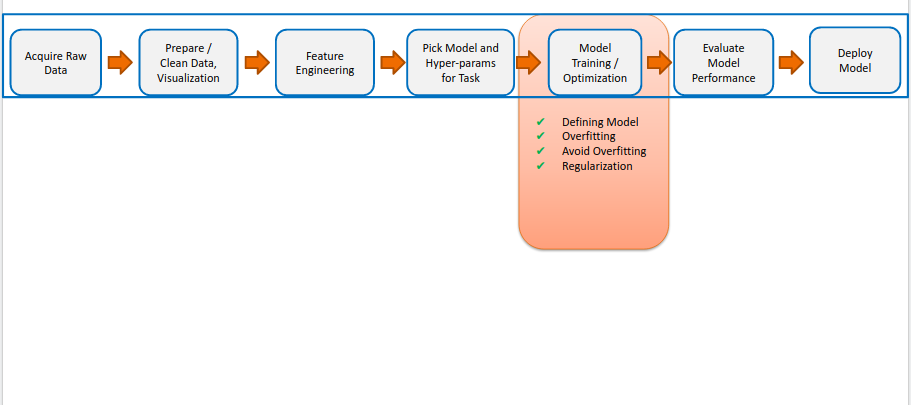
\includegraphics[width=1.015\textwidth, height=0.7\textheight]{Images/AIML_OFG_26.png}
\end{frame}

{\1
\begin{frame}
	\title{Thanks!!}
	\subtitle{Questions?}
	\maketitle
\end{frame}}


\end{document}

